\documentclass[]{ito}
% Paquetes de prueba
\usepackage{lipsum}

\autor{Ángel Isaac Fonseca Gómez}
\titulo{Framework para dispositivos IoT}
\director{NOMBRE DEL DIRECTOR}
\codirector{NOMBRE DEL CODIRECTOR}
\fecha{\today}
\keywords{MonogoDb, JavaScript, TypeScript, NodeJs, React, Backend, Frontend}
\palabras{MonogoDb, JavaScript, TypeScript, NodeJs, React, Backend, Frontend}

\graphicspath{ {imagenes/} }
\addbibresource{referencias.bib}

\includeonly{
    contenido/preambulo/resumen,
    contenido/preambulo/abstract,
    contenido/preambulo/introduccion,
    contenido/preambulo/planteamiento,
    contenido/preambulo/justificacion,
    contenido/preambulo/entrevista,
    contenido/preambulo/diagramafun,
    contenido/preambulo/objetivos,
    contenido/preambulo/modulos,
    contenido/preambulo/requerimientosfunc,
    contenido/preambulo/contribucion,
    contenido/capitulos/antecedentes,
    contenido/capitulos/estado,
    contenido/capitulos/metodologia,
    contenido/capitulos/resultados,
    contenido/epilogo/conclusiones,
    contenido/epilogo/recomendaciones,
    contenido/epilogo/productos,
    contenido/epilogo/anexos
}

\begin{document}

\maketitle

\tableofcontents
\listoffigures
\listoftables
\listofeqs

% Preambulo
\prechapter{RESUMEN}


\section{Introducción}
El proyecto \textbf{LIA} se centra en la monitorización de invernaderos utilizando luz artificial. Su objetivo es proporcionar una plataforma que permita a los usuarios controlar y optimizar el uso de recursos en entornos agrícolas mediante dispositivos IoT.

\section{Backend}
El backend está construido sobre un marco de trabajo especializado para dispositivos IoT, lo que permite la creación y gestión de modelos de datos adaptables a diferentes dispositivos. Esto incluye:

\begin{itemize}
    \item Generación de nuevos modelos de datos para dispositivos.
    \item Relación entre dispositivos y sus respectivos modelos de datos.
\end{itemize}

\section{Funcionalidades}
La plataforma LIA ofrecerá las siguientes funcionalidades:

\begin{itemize}
    \item Graficar datos en tiempo real para facilitar el análisis.
    \item Monitorizar el estado y rendimiento de los invernaderos.
    \item Crear y gestionar modelos de datos personalizados según las necesidades de los usuarios.
\end{itemize}

\section{Tecnologías}
Las tecnologías utilizadas en el desarrollo del proyecto incluyen:

\begin{itemize}
    \item \textbf{Node.js} y \textbf{Express} para el desarrollo del servidor.
    \item \textbf{TypeScript} y \textbf{JavaScript} para la lógica del backend y frontend.
    \item \textbf{React} para la construcción de interfaces de usuario interactivas.
    \item \textbf{MongoDB} como base de datos NoSQL para almacenar datos de dispositivos y modelos.
\end{itemize}

\makeatletter
\textbf{Palabras Clave:} \@palabras
\makeatother
% \lipsum[2-4]
\prechapter{ABSTRACT}
\large{El presente trabajo de tesis se centra en el desarrollo de una plataforma de monitorización para invernaderos de luz artificial, denominada \textbf{LIA}. Esta plataforma utiliza un backend basado en un marco de trabajo especializado para dispositivos IoT, lo que permite la creación y gestión de modelos de datos adaptables a diversos dispositivos de monitoreo. LIA ofrece funcionalidades para graficar y monitorizar en tiempo real los parámetros críticos de los invernaderos, así como para crear modelos de datos personalizados según las necesidades específicas de los usuarios. La implementación se lleva a cabo utilizando tecnologías modernas como Node.js, TypeScript, JavaScript, React y MongoDB. Este enfoque no solo optimiza el uso de recursos, sino que también mejora la toma de decisiones en la gestión de cultivos, contribuyendo así a la sostenibilidad y eficiencia en la agricultura de precisión.}


\makeatletter
\textbf{Keywords:} \@keywords
\makeatother
\prechapter{INTRODUCCIÓN}

\section{Introducción}

La agricultura de precisión ha revolucionado la forma en que se cultivan los productos agrícolas, optimizando el uso de recursos y maximizando la productividad. Uno de los desarrollos más prometedores en este ámbito es el uso de invernaderos de luz artificial, que permiten un control preciso sobre las condiciones de crecimiento, como la temperatura, la humedad y la iluminación. Sin embargo, la gestión eficiente de estos sistemas requiere herramientas avanzadas de monitorización y control, capaces de proporcionar datos en tiempo real y facilitar la toma de decisiones informadas.

El proyecto \textbf{LIA} se presenta como una solución innovadora para la monitorización de invernaderos de luz artificial. Su objetivo principal es desarrollar una plataforma que integre tecnologías de Internet de las Cosas (IoT) para la recolección y análisis de datos, permitiendo a los agricultores optimizar el funcionamiento de sus invernaderos. A través de la implementación de un backend robusto, se busca la capacidad de generar y gestionar modelos de datos que se adapten a las características de cada dispositivo de monitoreo, así como la capacidad de relacionar estos modelos con los dispositivos correspondientes.

\subsection{Objetivos del Proyecto}
Los objetivos específicos del proyecto LIA incluyen:

\begin{itemize}
    \item Desarrollar un sistema de monitorización que permita graficar en tiempo real los datos relevantes de los invernaderos.
    \item Crear un framework que facilite la gestión de modelos de datos personalizados para diferentes dispositivos IoT.
    \item Implementar una interfaz de usuario interactiva que permita a los agricultores acceder a información crítica sobre el estado de sus invernaderos.
    \item Proporcionar herramientas analíticas que ayuden en la toma de decisiones sobre el manejo de cultivos y recursos.
\end{itemize}

\subsection{Justificación}
La implementación de una plataforma como LIA es crucial en el contexto actual, donde la demanda de alimentos sigue aumentando debido al crecimiento poblacional y a los cambios en los patrones de consumo. La agricultura de luz artificial permite el cultivo durante todo el año y en diversas condiciones climáticas, pero su efectividad depende en gran medida de la capacidad de monitoreo y control que se tenga. Por lo tanto, LIA no solo contribuirá a mejorar la eficiencia y sostenibilidad de los invernaderos, sino que también permitirá a los agricultores adaptarse a las exigencias del mercado contemporáneo.

\subsection{Estructura del Documento}
El presente documento está estructurado de la siguiente manera: en la sección \textbf{2}, se abordarán las tecnologías empleadas en el desarrollo de la plataforma; la sección \textbf{3} describirá el diseño y la arquitectura del sistema; en la sección \textbf{4}, se presentarán los resultados obtenidos y se discutirán sus implicaciones; finalmente, la sección \textbf{5} concluirá con un resumen de los hallazgos y las futuras líneas de investigación.
\prechapter{PLANTEAMIENTO DEL PROBLEMA}

\section{Planteamiento del Problema}

El Tecnológico de Pabellón de Arteaga está llevando a cabo una investigación innovadora denominada \textbf{LIA}, cuyo objetivo es estudiar el crecimiento de plantas mediante el uso de luz artificial. Este proyecto busca optimizar las condiciones de cultivo y mejorar la eficiencia en el uso de recursos, lo que es fundamental en el contexto actual de la agricultura sostenible y la producción alimentaria.

Sin embargo, el proyecto LIA enfrenta una serie de desafíos en su fase de implementación. Actualmente, se utilizan dispositivos como la Raspberry Pi para la medición de variables del sistema, tales como la temperatura, la humedad y la intensidad de luz. Aunque estos dispositivos permiten la recolección de datos, la capacidad de análisis y gestión de dicha información es limitada. A medida que el proyecto crece, se hace necesario contar con un sistema robusto que facilite no solo la medición, sino también el almacenamiento, la monitorización en tiempo real y la visualización gráfica de los datos obtenidos.

El desarrollo de un \textbf{framework para dispositivos IoT} se presenta como la solución ideal para abordar estos problemas. Este framework permitirá:

\begin{itemize}
    \item \textbf{Almacenamiento de Datos}: Guardar de manera estructurada la información recolectada, lo que facilitará el acceso y la recuperación de datos históricos.
    \item \textbf{Monitorización en Tiempo Real}: Proporcionar a los investigadores herramientas que les permitan observar las variables del sistema al instante, mejorando la toma de decisiones y la respuesta ante variaciones.
    \item \textbf{Visualización Gráfica}: Ofrecer representaciones gráficas de los datos, lo que facilitará el análisis comparativo entre diferentes variables y condiciones experimentales.
\end{itemize}

Estos elementos son cruciales para el éxito del proyecto LIA, ya que no solo permitirán un control más efectivo del entorno de crecimiento, sino que también proporcionarán a los investigadores una plataforma que les permita realizar análisis más profundos y fundamentados. En consecuencia, el desarrollo de este framework será un paso determinante para la evolución del proyecto, permitiendo un enfoque más sistemático y científico en la investigación sobre el crecimiento de plantas con luz artificial.
\prechapter{JUSTIFICACIÓN}

\section{Justificación}

El desarrollo del proyecto \textbf{LIA} se fundamenta en la necesidad urgente de optimizar la producción agrícola en un mundo que enfrenta desafíos significativos en términos de seguridad alimentaria y sostenibilidad. A medida que la población global sigue creciendo, también lo hace la demanda de alimentos, lo que requiere que los métodos tradicionales de cultivo sean revisados y mejorados. La agricultura de precisión y el uso de tecnologías avanzadas, como la luz artificial y los sistemas de monitorización, se presentan como soluciones viables para abordar estos retos.

La justificación del proyecto LIA se puede desglosar en los siguientes puntos:

\subsection{Innovación en la Agricultura}
El uso de luz artificial para el crecimiento de plantas es un enfoque innovador que permite el cultivo en condiciones controladas, independientemente de factores climáticos externos. Esto no solo aumenta la eficiencia de la producción, sino que también permite el cultivo de variedades de plantas que de otro modo no prosperarían en ciertas regiones. La implementación de un sistema de monitorización y análisis de datos a través de un framework para dispositivos IoT permitirá maximizar los beneficios de esta tecnología.

\subsection{Mejora de la Toma de Decisiones}
El marco propuesto facilitará la recopilación y análisis de datos en tiempo real, lo que permitirá a los investigadores tomar decisiones informadas sobre el manejo de las variables del sistema. La capacidad de monitorizar condiciones como la temperatura, humedad e intensidad de luz, y visualizar estos datos en forma gráfica, contribuirá a una mejor comprensión de los efectos de diferentes parámetros en el crecimiento de las plantas. Esto es fundamental para la investigación científica y la mejora de los métodos de cultivo.

\subsection{Accesibilidad a la Información}
El desarrollo del framework no solo beneficiará a los investigadores del Tecnológico de Pabellón de Arteaga, sino que también tiene el potencial de ser una herramienta valiosa para otros institutos de investigación y agricultores. Al proporcionar acceso a datos estructurados y herramientas de análisis, el proyecto LIA contribuirá a la democratización del conocimiento en el ámbito de la agricultura de luz artificial.

\subsection{Sostenibilidad y Eficiencia}
La capacidad de monitorizar y controlar con precisión las variables ambientales en los invernaderos permitirá un uso más eficiente de los recursos, como el agua y la energía. Esto es especialmente relevante en un contexto global donde la sostenibilidad es una prioridad. La optimización de estos recursos no solo ayudará a reducir costos, sino que también contribuirá a la protección del medio ambiente.

\subsection{Contribución al Conocimiento Científico}
Finalmente, el proyecto LIA ofrecerá un marco sólido para la investigación y el desarrollo de nuevas tecnologías en el ámbito de la agricultura. La recopilación y análisis de datos proporcionarán una base empírica que podrá ser utilizada en estudios futuros, lo que contribuirá a un mejor entendimiento de las dinámicas del crecimiento de las plantas bajo luz artificial y abrirá nuevas líneas de investigación.

En resumen, la justificación del proyecto LIA radica en su capacidad para innovar en la agricultura, mejorar la toma de decisiones, facilitar el acceso a la información, promover la sostenibilidad y contribuir al conocimiento científico. Estas razones destacan la relevancia y la urgencia de llevar a cabo este proyecto en el contexto actual.
\prechapter{Entrevista}
\begin{itemize} 
    \item \textbf{¿Qué es lo que se quiere?} \ El propósito es desarrollar un sistema que permita monitorizar las variables de salida de los sensores del invernadero, que incluyen voltaje, potencia y amperaje. Estas son las principales variables que se medirán, y cada sensor se diferenciará por su nombre. Además, se busca la capacidad de graficar los datos según diferentes fechas o comparar los valores de distintos sensores en fechas específicas.

    \item \textbf{¿Quién será el usuario principal del sistema y cuál es su nivel de experiencia técnica?} \ Solo habrá un tipo de usuario. Se espera que los usuarios tengan una interacción sencilla con el sistema y que este sea fácil de entender, independientemente de su nivel de experiencia técnica.

    \item \textbf{¿Qué información necesitan los usuarios para tomar decisiones clave en el día a día?} \ La información que los usuarios necesitarán dependerá de las variables medidas (voltaje, potencia y amperaje), para poder analizar el estado del invernadero y tomar decisiones informadas basadas en los datos recolectados de los sensores.

    \item \textbf{¿Cómo se espera que los usuarios interactúen con el sistema?} \ Se espera que la interacción con el sistema sea simple y amigable, facilitando el acceso a la información necesaria sin complicaciones técnicas.

    \item \textbf{¿Qué tan crucial es el monitoreo en tiempo real para la operación del invernadero?} \ La monitorización en tiempo real es prioritaria para revisar el estado actual de los diferentes dispositivos del invernadero y poder tomar acciones oportunas si es necesario.

    \item \textbf{¿Cómo se deben gestionar y presentar las alertas críticas?} \ Las alertas críticas aún no están especificadas, pero se espera que el sistema tenga la capacidad de generarlas en caso de detectar anomalías importantes en los datos.

    \item \textbf{¿Se espera que el sistema no solo monitoree, sino que también automatice acciones en el invernadero?} \ No se espera que el sistema automatice acciones en el invernadero; su objetivo principal es el monitoreo y la visualización de datos.

    \item \textbf{¿Qué otros sistemas o herramientas están actualmente en uso y cómo se integraría el nuevo sistema?} \ Actualmente, no tienen ningún otro sistema en uso, por lo que el nuevo sistema será implementado desde cero sin necesidad de integración con herramientas existentes.

    \item \textbf{¿Hay alguna preferencia en cuanto a la tecnología o herramientas específicas para la implementación del sistema?} \ No existe preferencia hacia ninguna herramienta o tecnología en específico para la implementación del sistema.

    \item \textbf{¿Cuál es el presupuesto y el cronograma para la implementación del sistema?} \ [Aquí agregar la respuesta correspondiente] 
\end{itemize}
\prechapter{OBJETIVOS}
\section*{OBJETIVOS ESPECÍFICOS}
\addcontentsline{toc}{section}{OBJETIVOS ESPECÍFICOS}

\large{Implementar un sistema web de monitorización inteligente, con la opción de graficar la información para mejorar la comprensión de los datos brindados por los sensores.}\\[1cm]
\large{Con los siguientes objetivos específicos: }
\begin{itemize}
    \item Proveer fácil comprensión de los datos.
    \item Permitir revisión histórica de datos.
    \item Facilitar la fácil monitorización en tiempo real con los sensores.
    \item Acceso remoto al sistema.
    \item Generar modularización para facilitar el crecimiento.
\end{itemize}
\prechapter{CONTRIBUCIÓN AL CONOCIMIENTO}

\section{Contribución al Conocimiento}

El proyecto \textbf{LIA} tiene el potencial de realizar contribuciones significativas al campo de la agricultura y la investigación en tecnologías de iluminación artificial para el crecimiento de plantas. A continuación, se detallan las principales áreas en las que este proyecto contribuirá al conocimiento científico y práctico:

\subsection{Desarrollo de Modelos de Crecimiento}
El marco que se desarrollará como parte del proyecto LIA permitirá la creación de modelos de crecimiento más precisos y adaptativos para diversas especies de plantas bajo condiciones de luz artificial. Estos modelos no solo se basarán en datos empíricos recolectados a través de la plataforma, sino que también integrarán variables ambientales, lo que permitirá una comprensión más profunda de las interacciones entre estas variables y el crecimiento vegetal.

\subsection{Generación de Datos Estandarizados}
El proyecto facilitará la recolección de datos estandarizados y estructurados sobre el crecimiento de plantas bajo diferentes condiciones controladas. Esta recopilación sistemática de datos será valiosa para futuros estudios y permitirá la comparación entre investigaciones, promoviendo una base de conocimiento común que puede ser utilizada por otros investigadores en el área de la agricultura de precisión.

\subsection{Avances en Tecnología IoT}
El desarrollo del framework para dispositivos IoT no solo beneficiará al proyecto LIA, sino que también puede servir como modelo para futuras investigaciones en la aplicación de tecnologías IoT en la agricultura. Este enfoque permitirá una integración más fluida de dispositivos de monitoreo y control en otros sistemas agrícolas, fomentando el desarrollo de soluciones tecnológicas innovadoras en el sector.

\subsection{Educación y Capacitación}
El proyecto LIA también contribuirá al conocimiento a través de la educación y capacitación de estudiantes e investigadores en el uso de tecnologías de monitorización y análisis de datos. La experiencia adquirida por los participantes en el desarrollo y uso de la plataforma enriquecerá su formación y los preparará para futuros desafíos en el campo de la agricultura y la tecnología.

\subsection{Sostenibilidad Agrícola}
Al proporcionar datos y análisis que permitan optimizar el uso de recursos en la agricultura, el proyecto LIA contribuirá a la sostenibilidad en la producción agrícola. Los hallazgos derivados de la investigación pueden ayudar a establecer prácticas más eficientes que reduzcan el desperdicio y promuevan un uso responsable de los recursos, lo cual es fundamental para enfrentar los desafíos globales de seguridad alimentaria.

\subsection{Fomento de Investigaciones Futuras}
Finalmente, los resultados y datos generados por el proyecto LIA abrirán nuevas líneas de investigación en el campo de la agricultura y la tecnología de cultivo. Otros investigadores podrán utilizar estos datos como base para desarrollar estudios adicionales, contribuyendo así al avance del conocimiento en áreas relacionadas como la biotecnología, la genética de plantas y la agricultura sostenible.

\subsection{Proyecto Open Source}
Como parte de su compromiso con la difusión del conocimiento y la colaboración, el proyecto LIA será desarrollado como un proyecto open source. Esto permitirá que investigadores, desarrolladores y agricultores que requieran soluciones similares puedan acceder, modificar y contribuir a la plataforma, fomentando un ambiente de innovación y mejora continua. Además, el proyecto se exhibirá en el \textbf{COSS} (Centro de Observación y Sensores de Sostenibilidad) en Guadalajara en el año 2025, brindando visibilidad y oportunidades de colaboración con otros actores en el ámbito de la tecnología agrícola.

En resumen, el proyecto LIA no solo busca resolver problemas inmediatos relacionados con el crecimiento de plantas mediante luz artificial, sino que también se propone contribuir de manera significativa al acervo de conocimientos en el ámbito agrícola y tecnológico. Su impacto se extenderá más allá de los resultados inmediatos, fomentando un enfoque más científico y sistemático en la investigación y desarrollo agrícola.

\prechapter{Diagrama de funcionamiento}

\begin{figure}[ht]
    \centering
    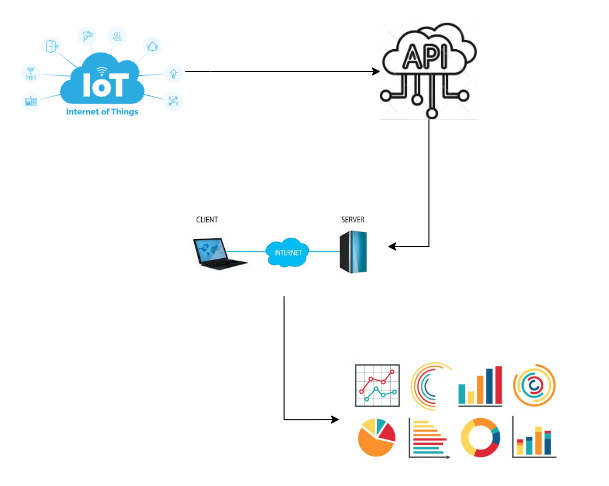
\includegraphics[width=0.8\textwidth]{imagenes/contenido/diagrama-fun.png}
    \caption{Diagrama de funcionamiento del proyecto}
    \label{fig:diagrama_funcionamiento}
\end{figure}
\prechapter{Modulos del sistema}

\section{Módulo de Usuarios}
\begin{table}[h!]
    \centering
    \begin{tabular}{|c|c|c|}
    \hline
    \rowcolor[HTML]{FCE8B2} 
    \textbf{Campo} & \textbf{Tipo de Dato} & \textbf{Descripción} \\ \hline
    ID & Entero & Identificador único del usuario. \\ \hline
    Nombre & Cadena de texto & Nombre completo del usuario. \\ \hline
    Nombre de Usuario & Cadena de texto & Nombre único de identificación del usuario. \\ \hline
    Correo Electrónico & Cadena de texto & Dirección de correo del usuario. \\ \hline
    Rol & Cadena de texto & Rol del usuario en el sistema (Admin, Usuario). \\ \hline
    Contraseña & Cadena de texto & Contraseña encriptada para acceder al sistema. \\ \hline
    Fecha de Creación & Fecha/Hora & Momento en que se creó el usuario. \\ \hline
    \end{tabular}
    \caption{Especificaciones del Módulo de Usuarios.}
\end{table}

\section{Módulo de Sensores}
\begin{table}[h!]
    \centering
    \begin{tabular}{|c|c|c|}
    \hline
    \rowcolor[HTML]{FCE8B2} 
    \textbf{Campo} & \textbf{Tipo de Dato} & \textbf{Descripción} \\ \hline
    ID & Entero & Identificador único del sensor. \\ \hline
    Módulo & Cadena de texto & Nombre del módulo al que pertenece el sensor. \\ \hline
    Sensores & Arreglo & Conjunto de sensores, cada uno con propiedades como: \\ \hline
    \hspace{5mm} Sensor & Cadena de texto & Tipo de sensor (Temperatura, Humedad, Luz). \\ \hline
    \hspace{5mm} Amp & Decimal & Valor de amperaje reportado por el sensor. \\ \hline
    \hspace{5mm} Volt & Decimal & Valor de voltaje reportado por el sensor. \\ \hline
    \hspace{5mm} Pot & Decimal & Valor de potencia reportado por el sensor. \\ \hline
    Fecha de Creación & Fecha/Hora & Momento en que se creó el registro del sensor. \\ \hline
    \end{tabular}
    \caption{Especificaciones del Módulo de Sensores.}
\end{table}

\section{Módulo de Graficación}
\begin{table}[h!]
    \centering
    \begin{tabular}{|c|c|c|}
    \hline
    \rowcolor[HTML]{FCE8B2} 
    \textbf{Campo} & \textbf{Tipo de Dato} & \textbf{Descripción} \\ \hline
    ID & Entero & Identificador único de la gráfica. \\ \hline
    Tipo de Gráfica & Cadena de texto & Tipo de visualización (Línea, Barras). \\ \hline
    Datos & JSON & Datos a graficar en formato JSON. \\ \hline
    Rango de Fechas & Fecha/Hora & Intervalo de tiempo para el que se generan los datos. \\ \hline
    Fecha de Creación & Fecha/Hora & Momento en que se creó el registro de la gráfica. \\ \hline
    \end{tabular}
    \caption{Especificaciones del Módulo de Graficación.}
\end{table}

\section{Módulo de Alertas}
\begin{table}[h!]
    \centering
    \begin{tabular}{|c|c|c|}
    \hline
    \rowcolor[HTML]{FCE8B2} 
    \textbf{Campo} & \textbf{Tipo de Dato} & \textbf{Descripción} \\ \hline
    ID & Entero & Identificador único de la alerta. \\ \hline
    Tipo de Alerta & Cadena de texto & Tipo de alerta (Crítica, Advertencia). \\ \hline
    Mensaje & Cadena de texto & Descripción de la alerta generada. \\ \hline
    Fecha de Generación & Fecha/Hora & Momento en que se generó la alerta. \\ \hline
    Estado & Cadena de texto & Estado de la alerta (Leída, No leída). \\ \hline
    \end{tabular}
    \caption{Especificaciones del Módulo de Alertas.}
\end{table}


\prechapter{Requerimientos}

Este capítulo describe los requerimientos que el sistema de monitorización de invernaderos debe cumplir para garantizar su correcta operación. Los requerimientos se dividen en dos secciones: funcionales y no funcionales, destacando aquellos que pueden ser medidos de manera objetiva.

\section{Requerimientos Funcionales y no funcionales}

% Ajuste el estilo de las tablas
\renewcommand{\arraystretch}{1.5} % Espacio entre filas

\begin{table}[h]
\centering
\begin{tabular}{|c|p{10cm}|c|}
\hline
\multicolumn{3}{|c|}{\textbf{Requerimiento Funcional}} \\ \hline
\textbf{RF-01} & \textbf{Almacenamiento de datos de los sensores:} El sistema guardará automáticamente los datos recolectados por los sensores, registrando valores como voltaje, amperaje y potencia. & \textbf{Versión 1.0} \\ \hline
\multicolumn{1}{|l|}{\textbf{Prioridad:}} MEDIA & \multicolumn{2}{l|}{\textbf{Dificultad:} MEDIA} \\ \hline
\end{tabular}
\caption{Requerimiento Funcional RF-01}
\end{table}
\vspace{1cm} % Espacio adicional

\begin{table}[h]
\centering
\begin{tabular}{|c|p{10cm}|c|}
\hline
\multicolumn{3}{|c|}{\textbf{Requerimiento Funcional}} \\ \hline
\textbf{RF-02} & \textbf{Consulta de sensores por área:} Los usuarios podrán consultar los datos de los sensores filtrados por áreas del invernadero, permitiendo obtener información específica de cada sección. & \textbf{Versión 1.0} \\ \hline
\multicolumn{1}{|l|}{\textbf{Prioridad:}} MEDIA & \multicolumn{2}{l|}{\textbf{Dificultad:} MEDIA} \\ \hline
\end{tabular}
\caption{Requerimiento Funcional RF-02}
\end{table}
\vspace{1cm} % Espacio adicional

\begin{table}[h]
\centering
\begin{tabular}{|c|p{10cm}|c|}
\hline
\multicolumn{3}{|c|}{\textbf{Requerimiento Funcional}} \\ \hline
\textbf{RF-03} & \textbf{Visualización gráfica de datos por fecha:} El sistema permitirá graficar los datos recolectados por los sensores en intervalos de fechas seleccionadas por el usuario, proporcionando una visualización clara de las tendencias. & \textbf{Versión 1.0} \\ \hline
\multicolumn{1}{|l|}{\textbf{Prioridad:}} MEDIA & \multicolumn{2}{l|}{\textbf{Dificultad:} MEDIA} \\ \hline
\end{tabular}
\caption{Requerimiento Funcional RF-03}
\end{table}
\vspace{1cm} % Espacio adicional

\begin{table}[h]
\centering
\begin{tabular}{|c|p{10cm}|c|}
\hline
\multicolumn{3}{|c|}{\textbf{Requerimiento Funcional}} \\ \hline
\textbf{RF-04} & \textbf{Visualización de los últimos datos de los sensores:} Los usuarios podrán consultar los datos más recientes recolectados por los sensores, mostrando la última información disponible en tiempo real. & \textbf{Versión 1.0} \\ \hline
\multicolumn{1}{|l|}{\textbf{Prioridad:}} MEDIA & \multicolumn{2}{l|}{\textbf{Dificultad:} MEDIA} \\ \hline
\end{tabular}
\caption{Requerimiento Funcional RF-04}
\end{table}
\vspace{1cm} % Espacio adicional

\begin{table}[h]
\centering
\begin{tabular}{|c|p{10cm}|c|}
\hline
\multicolumn{3}{|c|}{\textbf{Requerimiento Funcional}} \\ \hline
\textbf{RF-05} & \textbf{Graficación de múltiples sensores:} Los usuarios podrán seleccionar varios sensores para graficar sus datos simultáneamente, permitiendo la comparación de datos entre diferentes fechas. & \textbf{Versión 1.0} \\ \hline
\multicolumn{1}{|l|}{\textbf{Prioridad:}} MEDIA & \multicolumn{2}{l|}{\textbf{Dificultad:} MEDIA} \\ \hline
\end{tabular}
\caption{Requerimiento Funcional RF-05}
\end{table}
% Ajuste el estilo de las tablas
\renewcommand{\arraystretch}{1.5} % Espacio entre filas
\begin{table}[h]
\centering
\begin{tabular}{|c|p{10cm}|c|}
\hline
\multicolumn{3}{|c|}{\textbf{Requerimiento No Funcional}} \\ \hline
\textbf{RNF-01} & \textbf{Tiempo de respuesta del sistema:} El tiempo de respuesta para cargar cualquier vista no debe exceder los 2 segundos bajo condiciones normales de carga con hasta 50 usuarios simultáneos. & \textbf{Versión 1.0} \\ \hline
\multicolumn{1}{|l|}{\textbf{Prioridad:}} ALTA & \multicolumn{2}{l|}{\textbf{Dificultad:} MEDIA} \\ \hline
\end{tabular}
\caption{Requerimiento No Funcional RNF-01}
\end{table}
\vspace{1cm} % Espacio adicional

\begin{table}[h]
\centering
\begin{tabular}{|c|p{10cm}|c|}
\hline
\multicolumn{3}{|c|}{\textbf{Requerimiento No Funcional}} \\ \hline
\textbf{RNF-02} & \textbf{Escalabilidad del sistema:} El sistema debe escalar horizontalmente, soportando hasta 100 invernaderos adicionales sin que el tiempo de respuesta supere los 3 segundos. & \textbf{Versión 1.0} \\ \hline
\multicolumn{1}{|l|}{\textbf{Prioridad:}} ALTA & \multicolumn{2}{l|}{\textbf{Dificultad:} MEDIA} \\ \hline
\end{tabular}
\caption{Requerimiento No Funcional RNF-02}
\end{table}
\vspace{1cm} % Espacio adicional

\begin{table}[h]
\centering
\begin{tabular}{|c|p{10cm}|c|}
\hline
\multicolumn{3}{|c|}{\textbf{Requerimiento No Funcional}} \\ \hline
\textbf{RNF-03} & \textbf{Disponibilidad del sistema:} El sistema debe estar disponible el 99.9\% del tiempo, permitiendo un máximo de 8 horas de inactividad al año. & \textbf{Versión 1.0} \\ \hline
\multicolumn{1}{|l|}{\textbf{Prioridad:}} ALTA & \multicolumn{2}{l|}{\textbf{Dificultad:} MEDIA} \\ \hline
\end{tabular}
\caption{Requerimiento No Funcional RNF-03}
\end{table}
\vspace{1cm} % Espacio adicional

\begin{table}[h]
\centering
\begin{tabular}{|c|p{10cm}|c|}
\hline
\multicolumn{3}{|c|}{\textbf{Requerimiento No Funcional}} \\ \hline
\textbf{RNF-04} & \textbf{Seguridad de la información:} Toda la información transmitida deberá estar encriptada y cumplir con las regulaciones de protección de datos. & \textbf{Versión 1.0} \\ \hline
\multicolumn{1}{|l|}{\textbf{Prioridad:}} ALTA & \multicolumn{2}{l|}{\textbf{Dificultad:} MEDIA} \\ \hline
\end{tabular}
\caption{Requerimiento No Funcional RNF-04}
\end{table}


% Capitulos
\chapter{ANTECEDENTES}

\section{Antecedentes}

\subsection{Agricultura y Tecnología}
El avance de la tecnología ha tenido un impacto significativo en múltiples sectores, y la agricultura no ha sido la excepción. A lo largo de las últimas décadas, el concepto de \textbf{agricultura de precisión} ha ganado tracción, al integrarse con tecnologías emergentes como el Internet de las Cosas (IoT), sensores inteligentes y análisis de grandes volúmenes de datos (big data). Estas innovaciones han permitido mejorar la eficiencia en la producción agrícola, reducir el uso de recursos naturales y optimizar las condiciones para el crecimiento de las plantas. Sin embargo, uno de los grandes retos a los que se enfrenta la agricultura es la sostenibilidad en áreas de cultivo con acceso limitado a luz natural. Aquí es donde la \textbf{iluminación artificial} ha comenzado a jugar un papel clave.

\subsection{El Uso de la Iluminación Artificial en la Agricultura}
La luz es un factor crucial para la fotosíntesis, el proceso que permite a las plantas transformar la energía lumínica en compuestos químicos necesarios para su crecimiento. En muchos entornos controlados, como los invernaderos, la luz natural no siempre es suficiente para asegurar un crecimiento óptimo, lo que ha llevado al uso de \textbf{luz artificial} como complemento o sustituto. A medida que se han desarrollado nuevas tecnologías de iluminación, como las luces LED ajustables en longitud de onda, los invernaderos han podido recrear condiciones óptimas de luz para distintas especies vegetales. La capacidad de manipular el espectro lumínico ha permitido optimizar el crecimiento en condiciones que anteriormente eran inviables, promoviendo así un crecimiento más controlado y eficiente.

\subsection{Investigaciones Previas}
En los últimos años, se han llevado a cabo diversos estudios que exploran los efectos de la luz artificial en el crecimiento de plantas. Investigaciones como las de \textit{Smith et al.} (2020) y \textit{González et al.} (2019) han demostrado que ajustar los niveles de luz y la longitud de onda puede impactar directamente en el ciclo de crecimiento de varias especies. Sin embargo, la mayoría de estas investigaciones se han centrado en entornos experimentales y no en la aplicación a gran escala con tecnologías de IoT para la monitorización en tiempo real. Además, aunque se han logrado avances en sistemas de monitorización, aún existe una brecha en la integración de dispositivos IoT que permitan analizar y gestionar eficientemente las variables del entorno que influyen en el crecimiento vegetal, tales como la temperatura, la humedad y la cantidad de luz recibida.

\subsection{Internet de las Cosas (IoT) en la Agricultura}
El \textbf{Internet de las Cosas} (IoT, por sus siglas en inglés) ha emergido como una de las tecnologías clave para la transformación digital de la agricultura. IoT se refiere a la interconexión de dispositivos y sensores inteligentes a través de Internet, lo que permite la captura de datos en tiempo real y la automatización de procesos. En el contexto agrícola, los dispositivos IoT pueden monitorizar múltiples variables, como la temperatura del suelo, la humedad, los niveles de luz, y otros factores críticos para el crecimiento de las plantas. La capacidad de tomar decisiones informadas basadas en datos recolectados en tiempo real no solo mejora la eficiencia, sino que también reduce los costos y minimiza el impacto ambiental.

Varios proyectos a nivel mundial han utilizado IoT para optimizar la producción agrícola. Por ejemplo, en \textit{Xiang et al.} (2021) se desarrolló un sistema de sensores integrados para invernaderos, lo que permitió ajustar automáticamente las condiciones ambientales en función de los datos recolectados. Este enfoque de monitoreo inteligente es cada vez más relevante para maximizar la productividad en espacios controlados como los invernaderos.

\subsection{Proyecto LIA y Tecnológico de Pabellón de Arteaga}
El \textbf{Tecnológico de Pabellón de Arteaga} ha lanzado una iniciativa llamada \textbf{LIA (Luz Artificial para la Agricultura)}, cuyo objetivo es investigar y desarrollar tecnologías que mejoren el crecimiento de las plantas utilizando iluminación artificial. Esta iniciativa surge ante la necesidad de crear entornos controlados donde la luz natural no sea el principal recurso para la fotosíntesis. Como parte de este proyecto, se busca implementar un sistema de monitorización inteligente que utilice una combinación de dispositivos IoT, como \textbf{Raspberry Pi}, para medir variables ambientales y controlar el sistema de iluminación. El reto, sin embargo, radica en la integración de estos dispositivos en una plataforma robusta que permita analizar, graficar y gestionar los datos generados por los sensores.

La integración de iluminación artificial en la agricultura ha mostrado grandes beneficios, especialmente en entornos donde la luz natural es insuficiente para las necesidades de las plantas. ("Estudios recientes han demostrado que la manipulación del espectro de luz puede afectar el crecimiento de las plantas") \cite{gonzalez2019, zhang2021}. ("Las luces LED, con la capacidad de ajustar su espectro lumínico, ofrecen nuevas oportunidades para la agricultura moderna") \cite{zhang2021}.

\subsection{Framework para Dispositivos IoT}
Como solución a esta problemática, se plantea el desarrollo de un \textbf{framework para dispositivos IoT}, diseñado específicamente para monitorear las variables ambientales en los invernaderos. Este framework permitirá no solo la captura y almacenamiento de datos en tiempo real, sino también la creación de modelos personalizados para los dispositivos que monitoricen los parámetros de crecimiento de las plantas. Gracias a su flexibilidad, los investigadores podrán adaptar el sistema a las necesidades específicas de cada especie vegetal, facilitando la toma de decisiones en el manejo de los cultivos.

El framework está diseñado para ser escalable y abierto, por lo que podrá ser utilizado por otros proyectos que requieran soluciones similares. Su arquitectura se basa en tecnologías modernas como \textbf{Node.js}, \textbf{TypeScript}, \textbf{MongoDB}, y \textbf{React}, asegurando un alto rendimiento y una experiencia de usuario interactiva. Además, se espera que este framework pueda ser implementado en otros entornos agrícolas o industriales donde la monitorización en tiempo real de variables críticas sea indispensable.


\subsection{Conclusión}
A través de estos antecedentes, se ha establecido el contexto necesario para comprender la relevancia del proyecto LIA. La integración de la tecnología IoT en la agricultura no solo aborda problemas relacionados con la eficiencia y la productividad, sino que también contribuye a la sostenibilidad agrícola en un mundo donde el acceso a recursos naturales es cada vez más limitado. El proyecto LIA se propone como una solución tecnológica innovadora que permitirá a los investigadores y agricultores monitorear en tiempo real las condiciones de crecimiento, contribuyendo al avance de la agricultura moderna y sostenible.
("Por otro lado, los frameworks de IoT han evolucionado para ofrecer soluciones modulares y escalables, permitiendo la creación de modelos personalizados de monitoreo y control para distintas aplicaciones, incluidos los sistemas agrícolas") \cite{lopez2020, fernandez2021}

\chapter{ESTADO DEL ARTE}

\lipsum[1-2]

Aqui podemos ver una cita que extrae el nombre del autor: \citeauthor{latex:companion}

\chapter{METODOLOGÍA}

\lipsum[1-1] \parencite{latex2e}

En la \autoref{tab:tabla1} podemos observar un ejemplo de tabla.

\begin{table}[H]
	\centering
	\caption{Mi tabla}\label{tab:tabla1}
	\begin{tabular}{@{}llr@{}}
		\toprule
		\multicolumn{2}{c}{Item} &                          \\ \cmidrule(r){1-2}
		Animal                   & Description & Price (\$) \\ \midrule
		Gnat                     & per gram    & 13.65      \\
		                         & each        & 0.01       \\
		Gnu                      & stuffed     & 92.50      \\
		Emu                      & stuffed     & 33.33      \\
		Armadillo                & frozen      & 8.99       \\ \bottomrule
	\end{tabular}
\end{table}

Este es un ejemplo de una referencia \autoref{noexiste} y de una cita\autocite{noexiste} no encontradas.
\chapter{RESULTADOS}

\lipsum[1-1]\autocite{texbook,latex:companion}.

En la \autoref{fig:fig2} podemos observar un ejemplo de figura.

\begin{figure}[H]
	\centering
	
\includegraphics[width=\textwidth,height=0.3\textwidth]{overleaf}
	\caption{Mi figura}\label{fig:fig2}
\end{figure}

En la \autoref{eq:ecuacion1} podemos observar un ejemplo de ecuación.

\begin{eq}[H]
	\caption{Mi ecuación}\label{eq:ecuacion1}
	\[
		\mathcal L_{\mathcal T}(\vec{\lambda})
		= \sum_{(\mathbf{x},\mathbf{s})\in \mathcal T}
		\log P(\mathbf{s}\mid\mathbf{x}) - \sum_{i=1}^m
		\frac{\lambda_i^2}{2\sigma^2}
	\]
\end{eq}

% Ejemplo de una Figura en otra página se puede ver en la \vref{fig:fig3}

% \begin{figure}[H]
% 	\centering
% 	\includegraphics[width=\textwidth,height=0.5\textwidth]{example-image}
% 	\caption{Figura en otra página}\label{fig:fig3}
% \end{figure}

Este es un ejemplo de matemática dentro de línea \(x^2 + y^2 = z^2\).

% Este es el ejemplo de una cita múltiple \autocite{texbook,latex:companion}.

% Epilogo
\prechapter{CONCLUSIONES}

\lipsum[1-2] \parencite{lesk:1977}

\prechapter{RECOMENDACIONES}

\lipsum[1-2]

\printbibliography[title={REFERENCIAS BIBLIOGRÁFICAS},heading=bibintoc]

\prechapter{PRODUCTOS ACADÉMICOS}

\lipsum[1-1]
\prechapter{ANEXOS}

\lipsum[1-3]





\end{document}